%\documentclass[10pt, twocolumn]{article}
\documentclass[twocolumn,showpacs,preprintnumbers,amsmath,amssymb,prd]{revtex4}
%\documentclass[11 pt,preprint,preprintnumbers,amsmath,amssymb, prd]{revtex4}

% Preamble adapted from Surjeet Rajendran

\usepackage{latexsym}
\usepackage{amssymb}
\usepackage{epsfig,amsmath,graphics}
\usepackage{epstopdf}
\usepackage{verbatim}
\usepackage{wasysym}
\usepackage{hyperref}
\usepackage{feynmp-auto} % feynman diagrams
%\usepackage{subfig}
\usepackage[utf8]{inputenc}
\usepackage{xpatch}
\usepackage{xcolor}
\hypersetup{
    colorlinks,
    linkcolor={red!80!black},
    citecolor={green!60!black},
    urlcolor={blue!60!black}
}
\usepackage{appendix}

\newcommand{\Ez}{\mathcal{E}_0}

\newcommand{\OO}{\mathcal{O}}
\newcommand{\LL}{\mathcal{L}}
\newcommand{\HH}{\mathcal{H}}

\newcommand{\GeV}{\text{GeV}}
\newcommand{\MeV}{\text{MeV}}
\newcommand{\keV}{\text{keV}}
\newcommand{\rad}{\text{rad}}
\newcommand{\cm}{\text{cm}}
\newcommand{\angstrom}{\buildrel _{\circ} \over {\mathrm{A}}}
\newcommand{\pslash}{p\hspace{-0.070in}/\,}
\newcommand{\Mpl}{M_{\text{pl}}}
\newcommand{\ket}[1]{\ensuremath{\left|#1\right>}}
\newcommand{\bra}[1]{\ensuremath{\left<#1\right|}}
\newcommand{\braket}[2]{\ensuremath{\left<#1|#2\right>}}
%Large Parentheses
\def\r{\right)}
\def\l{\left(}

\begin{document}

\title{White Dwarfs as Dark Matter Detectors}

\author{Ryan Janish}
\affiliation{Berkeley Center for Theoretical Physics, Department of Physics,
University of California, Berkeley, CA 94720, USA}

\author{Vijay Narayan}
\affiliation{Berkeley Center for Theoretical Physics, Department of Physics,
University of California, Berkeley, CA 94720, USA}

\author{Surjeet Rajendran}
\affiliation{Berkeley Center for Theoretical Physics, Department of Physics,
University of California, Berkeley, CA 94720, USA}

\author{Paul Riggins}
\affiliation{Berkeley Center for Theoretical Physics, Department of Physics,
University of California, Berkeley, CA 94720, USA}

\begin{abstract}

White dwarfs can serve as detectors for ultra-heavy dark matter states which interact to trigger type Ia supernovae.
This was originally proposed in \cite{Graham:2015apa} and used to place bounds on primordial black holes.
In this paper we extend the capability of white dwarf detectors to dark matter candidates with non-gravitational couplings, focusing on collisions, decays, and transits within the white dwarf.
In particular, we provide a detailed analysis of the explosiveness for any heating mechanism in the white dwarf which releases high-energy standard model particles.
As an example, we apply this to constrain supersymmetric Q-ball dark matter in a vast region of parameter space fundamentally inaccessible to terrestrial-based experiments.


\end{abstract}
\maketitle
\tableofcontents

\section{Introduction}
\label{sec:Introduction}

The detection of ultra-heavy dark matter (DM) is an open problem which will ultimately require a confluence of astrophysical probes.
For instance, DM masses above $\sim 10^{22} ~\GeV$ will register fewer than a single event per year in a typical terrestrial detector of size $\sim (100 ~\text{m})^2$.
Furthermore, the lack of conclusive signatures on a variety of experimental fronts has led many to consider DM candidates far above the weak scale and their potential signatures \textcolor{blue}{cite people}.
One possibility proposed by \cite{Graham:2015apa} is that ultra-heavy DM can trigger supernovae (SN) in sub-Chandrasekhar white dwarf (WD) stars by inducing runaway fusion.
In this regard, white dwarfs can serve as detectors for ultra-heavy DM states.

White dwarfs are particularly suited to this task as they are more susceptible to runaway fusion than are main-sequence stars.
Runaway fusion requires that two criteria be met: a region within the star must be hot enough to support exothermic fusion reactions, and the rate at which energy is released must dominate any cooling mechanisms that drain energy from the fusing region.
Since the pressure of a WD is set by electron degeneracy and is thus independent of temperature, thermal expansion is suppressed as a potential cooling mechanism.
Therefore WD cooling relies on thermal diffusion, which becomes less important over longer length scales, and can be overcome by sufficiently heating a large enough region of the WD.

The necessary trigger for runaway fusion was initially computed in \cite{Woosley} and recently implemented in \cite{Graham:2015apa} to constrain primordial black holes, which can ignite WD stars via gravitational dynamical friction.
In addition, the authors of \cite{Graham:2015apa} identify several other heating mechanisms involving DM which may be constrained in a similar manner.
In this work, we extend their analysis to DM candidates with non-gravitational couplings, focusing DM-DM collisions, DM decays, and DM transits in a WD which release energy in the form of standard model (SM) particles.
More generally, we provide a detailed analysis of the explosive nature and resulting constraints on any DM with interactions of this sort.
DM candidates with interactions of this type include baryonic Q-balls found in supersymmetric extensions of the SM and models of dark nuclei with higher-dimension couplings to the SM.
The general constraints that follow will come from either observing specific long-lived white dwarfs or comparing the measured type Ia SN rate with the expected rate due to DM events.
As a concrete example, we are able to constrain Q-ball DM in regions of parameter space fundamentally inaccessible to terrestrial experiments.
However, it is important to note that any such DM constraints are by nature complimentary to terrestrial ones - it is more massive DM that is likely to trigger SN, and also more massive DM that have sufficiently low flux on Earth.
What allows the WD ``detector" to be effective in this regime is its enhanced surface area $\sim (10^4 ~\text{km})^2$, exceptionally long lifetime $\sim \text{Gyr}$, and astronomical abundance in the galaxy. 

We begin in Section~\ref{sec:Review} by reviewing the conditions for runaway fusion in a WD.
The ability for such interactions to trigger supernovae will be determined by a heating length, which is computed in Section~\ref{sec:SMHeating} for different SM particles and energies. 
In Section~\ref{sec:DMexplode}, we parametrize the properties of DM necessary to ignite white dwarfs through non-gravitational interactions. 
Following this general discussion, we apply the WD detector to place constraints on ultra-heavy DM in Section~\ref{sec:Constraints}, and apply these constraints in Section~\ref{sec:QBalls} to Q-balls.
We conclude in Section~\ref{sec:discussion}.

\section{White Dwarf Runaway Fusion}
\label{sec:Review}

Any process which deposits energy in a WD will eventually heat a localized region within the star. 
Since we are interested in nuclear fusion, let $L_0$ be the length scale of the local peak in ion temperature $T_0$ and $\Ez \sim T_0 n_\text{ion} L_0^3$ be the excess thermal energy it contains, where $n_\text{ion}$ is the number density of ions. 
Note that the size and thermal properties of any heated region will evolve in time, so we take $L_0$ and $\Ez$ to characterize this peak as it initially forms, i.e.\ immediately after a temperature profile for ions has been established.
Thus for a given heating event, $L_0$ is a measure of the efficiency with which the energy deposit is transferred to ions in the stellar medium.
This may vary significantly with the form of the energy deposit and with WD density.
For example, suppose that kinetic energy is transferred directly to a single ion through a short-range elastic scatter.
This ion would thermalize with neighboring ions, resulting in a heating length $L_0$ of order the ion mean free path.
In the other extreme, suppose that a process produces electrons in the WD at energies just above the Fermi energy.
These electrons have Pauli-suppressed interactions and will travel a long distance before their energy is scattered and thermalized among ions, resulting in a much larger $L_0$.

The fate of a locally heated region in a WD is either a nonviolent diffusion of the energy deposit across the star, or a runaway fusion chain-reaction that will destroy the star.
The precise outcome is governed by two parameters: the fusion temperature $T_f$ and trigger size $\lambda_T$.
The fusion temperature $T_f$ is the threshold for the onset of fusion and is given by the energy required for ions to overcome their mutual Coulomb barrier.
In carbon-oxygen WDs, this is a constant $T_f \sim \MeV$. \textcolor{blue}{citation?}
However, while any region with $T_0 > T_f$ will initially support fusion, this condition is not sufficient for triggering a runaway process.
Sustained heating through nuclear fusion can only be maintained if the timescale for cooling is consistently longer than the timescale for heating. 
Cooling in a WD is dominated by diffusion \textcolor{blue}{citation?} and the characteristic diffusion time for a heated region increases with its size while the rate of fusion is independent of size. 
Therefore, there will always be a critical size of a heated region (at fixed temperature) above which fusion is maintained as the dominant thermal process.
For a region at the threshold of nuclear fusion $T_f$, this condition defines the trigger size $\lambda_T$.
The value of $\lambda_T$ is highly dependent on stellar density, and is set by either the thermal diffusivity of photons or degenerate electrons.
It has been calculated numerically in \cite{Woosley} and analytically scaled for varying WD masses in \cite{Graham:2015apa}.
As in \cite{Graham:2015apa}, we restrict our attention to carbon-oxygen WDs in the upper mass range $\sim 0.7 - 1.4 ~M_{\odot}$ which correspond to a central number density of ions $n_\text{ion} \sim 10^{29} - 10^{32} ~\cm^{-3}$.
Over this range, the trigger size is approximately $\lambda_T \sim 10^{-5} - 10^{-2} ~\text{cm}$.

In summary, a local temperature peak $T_f$ in a WD will either always be dominated by diffusive cooling if $L_0 < \lambda_T$ or sustained fusion if $L_0 > \lambda_T$.  
However, there is an additional possibility if $T_0 > T_f$ that the thermal evolution is initially dominated by diffusion but at a later time results in runaway fusion. 
We can assess this outcome by assuming the region with $T_0 > T_f$ begins to diffuse and cool until its temperature reaches $\sim T_f$.
If the size of the region at this point is larger than $\lambda_T$, a runaway will occur.  
For a heated region of initial size $L_0$ and total energy deposit $\Ez$, the condition to trigger a type Ia SN via runaway fusion is
\begin{equation}
\label{eq:boom}
  \Ez \gtrsim n_\text{ion} T_f \text{max}\{L_0, \lambda_T\}^3.
\end{equation}
This implies the explosion condition used in \cite{Graham:2015apa}, but also provides a less stringent criteria applicable to regions of temperature greater than $T_f$ and size less than $\lambda_T$ which was not needed in that work.  
Thus there is an absolute minimum energy required to ignite a WD
\begin{equation}
\label{eq:Eboom}
\mathcal{E}_{\text{boom}} \sim n_\text{ion} T_f \lambda_T^3 \sim 10^{15} - 10^{22} ~\GeV,
\end{equation}
where $\mathcal{E}_{\text{boom}} $ varies with trigger size $\lambda_T$ over the range of WD densities.
This is plotted in Figure \ref{fig:Eboom}.
Note that the threshold \eqref{eq:Eboom} is only sufficient if the deposited energy thermalizes within a region of size $L_0 < \lambda_T$.
The threshold energy for explosion is parametrically larger if energy is deposited on a larger length scale $L_0 > \lambda_T$.
As a result, understanding the heating length $L_0$ of a process is critical to determining whether or not it is capable of destroying a WD. 

\begin{figure}
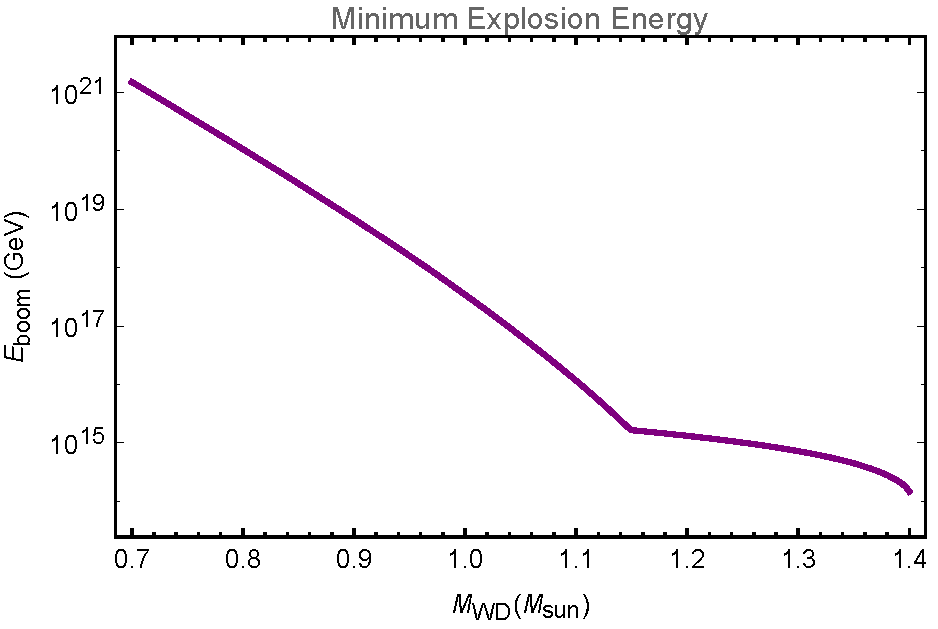
\includegraphics[scale=.45]{Eboom.pdf}
\caption{Minimum energy required to trigger SN as a function of WD mass, based on numerical results for $\lambda_T$ \cite{Woosley}.}
\label{fig:Eboom}
\end{figure}

\section{Dark Matter and Non-Gravitational Heating of a White Dwarf}
\label{sec:SMHeating}

Having reviewed the conditions necessary for an energy deposit to initiate runaway fusion in a WD, we turn our attention towards heating events induced by DM. 
A DM encounter with a WD must transfer energy to ions, as characterized by the heating length $L_0$ and total energy deposit $\Ez$ for the process, such that \eqref{eq:boom} is satisfied. 
Of course, the heating of a WD due to such an encounter will necessarily depend on the nature of the DM and must be explicitly calculated for a given DM model. 
This was done in \cite{Graham:2015apa} for the simple case of primordial black holes which transit a WD and locally heat the star through gravitational dynamical friction. 
However, non-gravitational interactions also have the potential to trigger SN. 
In particular, any DM candidate which couples to the SM will generically be able to release SM secondaries though some effective interaction as depicted in Figure \ref{fig:feynman}. 
For these types of processes, the unknown DM physics only serves to determine the initial distribution in space, momentum, and species of the SM particles produced in the star, while the actual heating proceeds entirely though known SM interactions. 
It is therefore necessary to understand how energy is transferred from SM particles to the stellar medium in order to assess the explosiveness of a more general non-gravitational DM-WD encounter. 

\begin{figure}
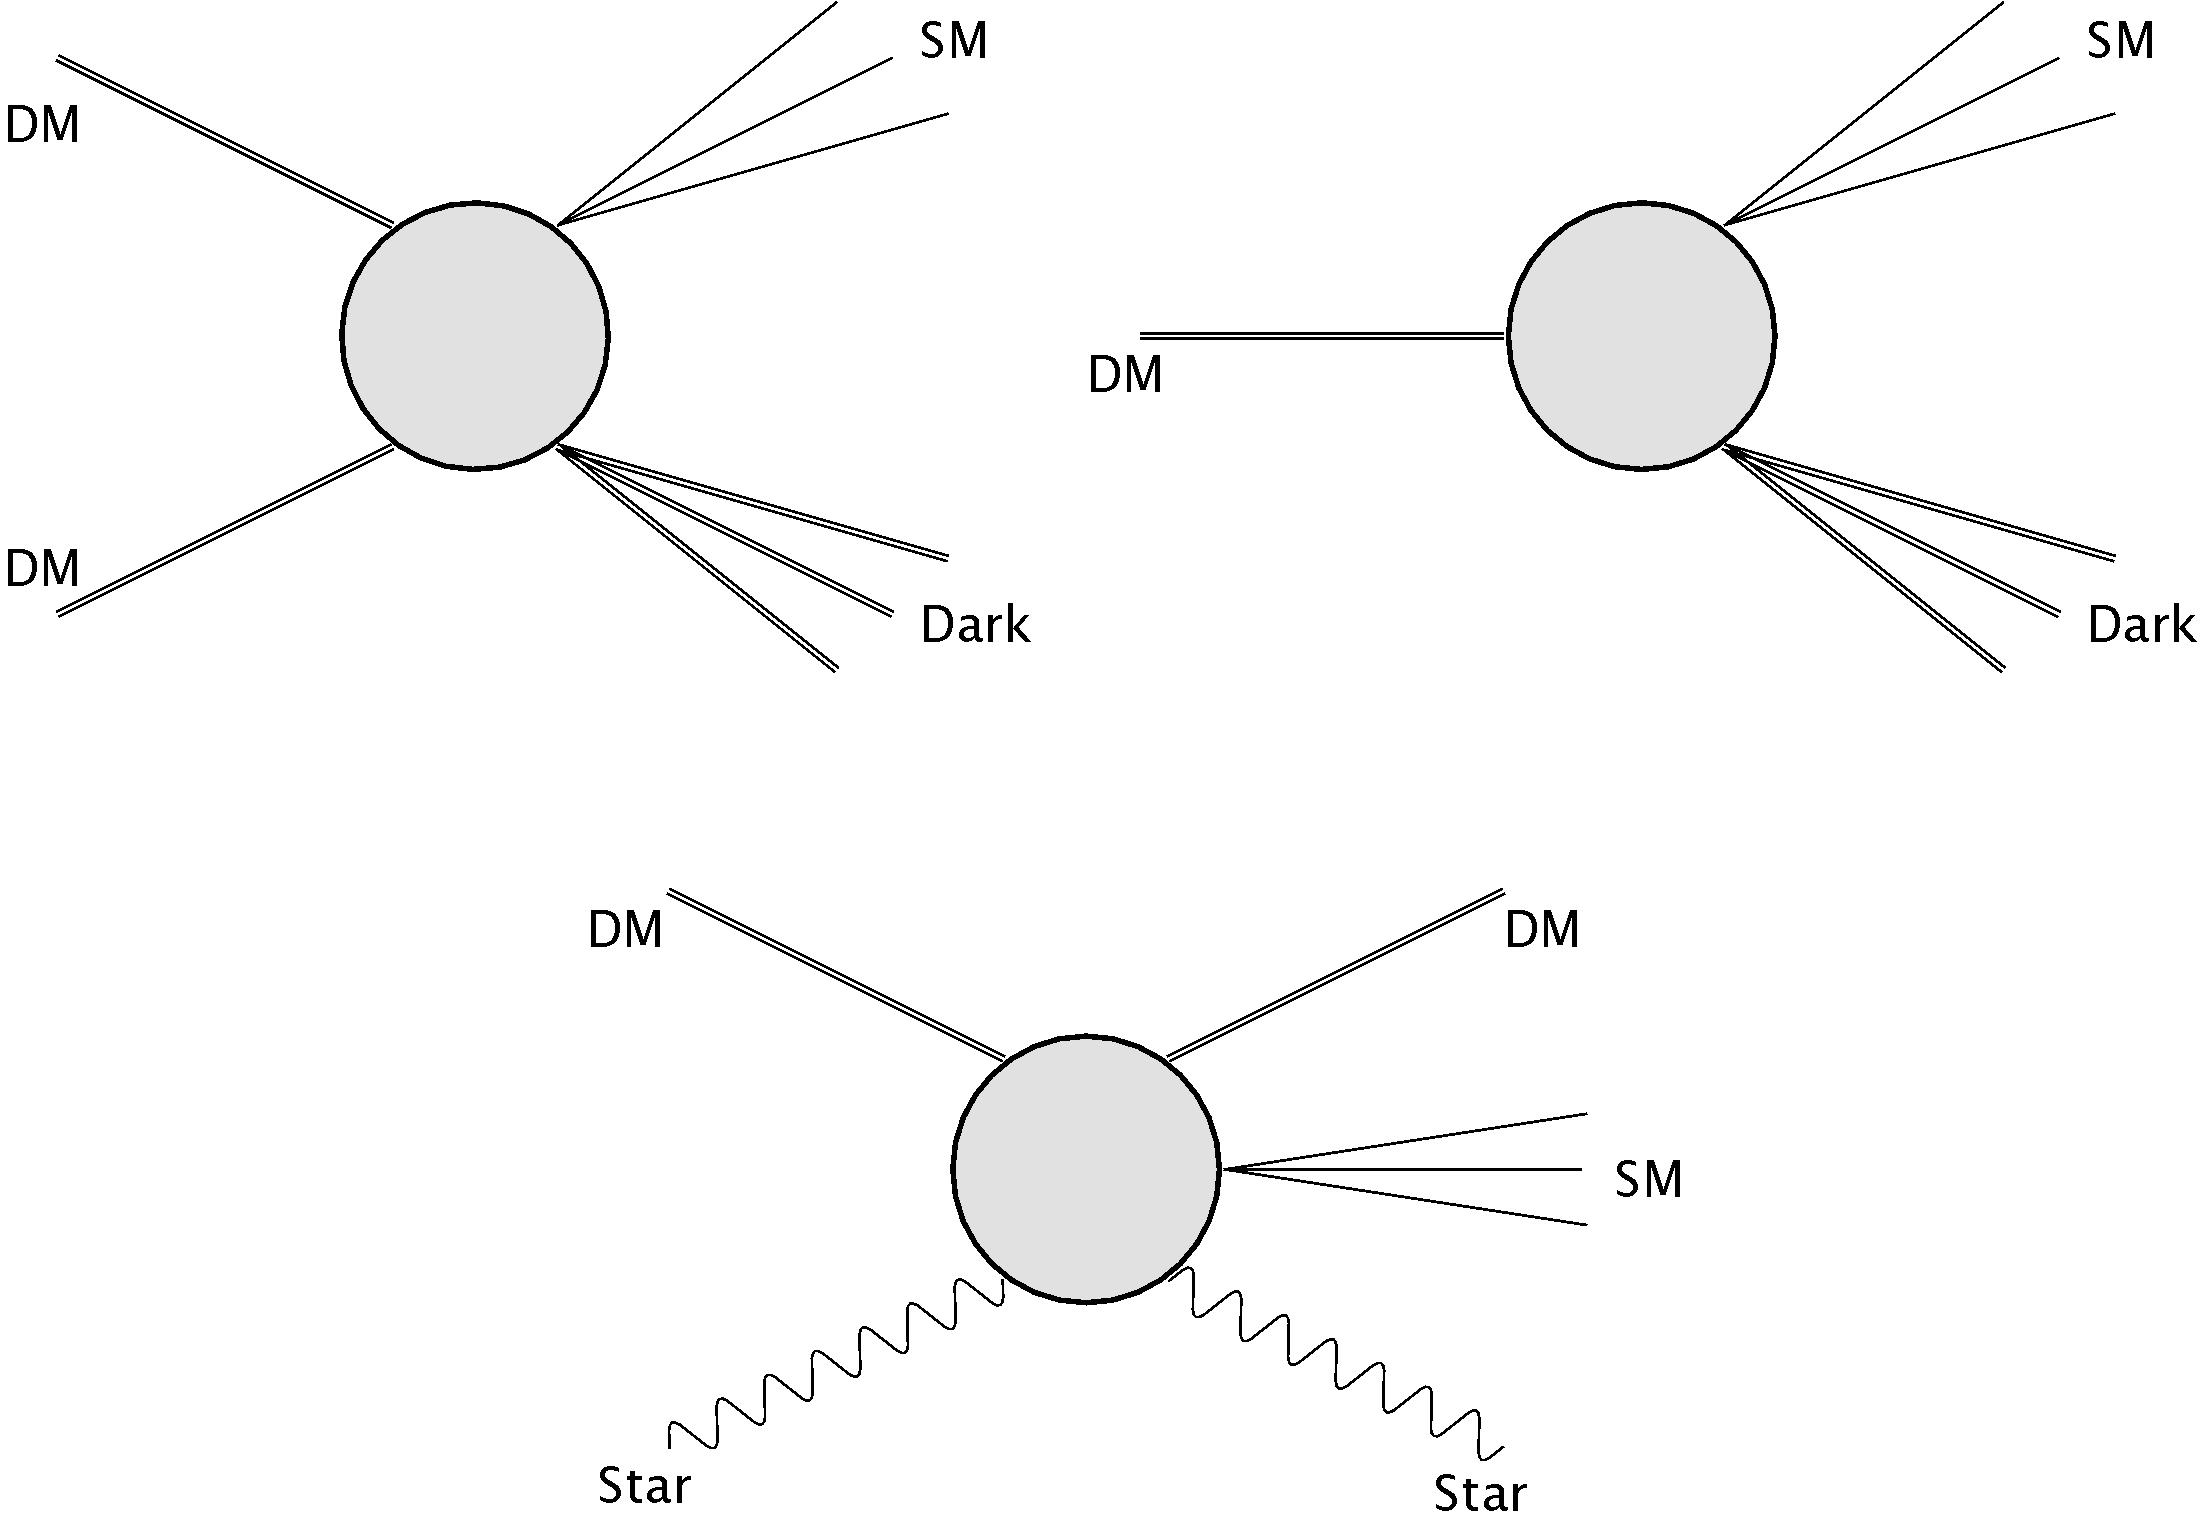
\includegraphics[scale=0.09]{feynmandiag.jpg}
\caption{Schematic of possible non-gravitational DM interactions in a WD. Heating of the WD occurs through SM particle production - also depicted are potential dark sector states involved in any such interaction.}
\label{fig:feynman}
\end{figure}

The remainder of this section is dedicated to the heating properties of individual SM particles of given energy $\epsilon$ and species $i$. 
As we are only concerned with depositing sufficient energy to initiate runaway fusion, we take $\epsilon \gtrsim T_f \sim \text{MeV}$.
\textcolor{blue}{We also assume a nominal upper bound $\epsilon \lesssim 10^{17} ~\GeV$ so that we may conservatively ignore interactions beyond the SM.} 
The heating due to a single released SM particle is most accurately described by the shape of the resulting temperature profile, which we parameterize by two length scales: the displacement $R_i(\epsilon)$ of the center of the profile from the starting location of the SM particle, and the width $\Delta_i(\epsilon)$ of the temperature peak.  
Note that $R_i \gtrsim \Delta_i$ is always true although for most species, $R_i \sim \Delta_i$ with neutrinos being the one (unsurprising) exception.
Either of these quantities may be relevant in determining the heating length of a general DM-WD encounter depending on their relative sizes and on the number of SM particles involved.  
Finally, an essential ingredient for calculating $R_i$ and $\Delta_i$ is the stopping power of high-energy SM particles in the WD medium. 
We will summarize here as needed the dominant sources of energy loss for each species while a more detailed analysis is provided in Appendix \ref{sec:appendix}. 


% We will primarily focus on the many-secondary case, as heating by one particle requires individual particle energies of $\epsilon \gtrsim \mathcal{E}_\text{boom} \gtrsim 10^15 \GeV$, which begins the approach the bounds of our interaction confidence $\epsilon \lesssim 10^{17} ~\GeV$
% In addition, for secondary species with $\Delta_i \sim R_i$, an encounter that deposits the same total energy by releasing more secondaries of less individual energy will always be more explosive than encounters that focus the deposited energy into fewer secondaries. 



\subsection{Heating Properties: Hadrons}
The stopping powers for nucleons and pions in a WD are depicted in Figures \ref{fig:SPnuc} and \ref{fig:SPpion}.
\textcolor{blue}{add elastic nuclear scattering lines to these plots}
In terrestrial detectors at the energies, the stopping powers would be dominated by Coulomb scattering of atomic electrons, however in the WD scattering of electrons is suppressed by degeneracy and efficient charge screening.
For energies greater than the typical nuclear binding energy $E_N \sim 10 ~\text{MeV}$, the energy loss for all hadrons is dominated by inelastic nuclear collisions. 
The collisions produce a lighter, excited nucleus and a few outgoing hadrons which roughly carry away the incident particle's kinetic energy in equal fractions. \textcolor{blue}{citation}
If these secondary hadrons have energy above $E_N$, they too are predominantly stopped by inelastic nuclear collisions, producing a roughly collinear shower. 
As each collision divides the incoming energy equally among a few products, energy of the shower constitutions is decaying via a stopping power
\begin{equation}
  \l \frac{dE}{dx} \r \sim \frac{E}{l_\text{h,inel}}. 
\end{equation}
Where $l_\text{h,inel}$ is the mean free path for inelastic hadron-nuclei collisions.
The shower terminates when the constituents reach engery $E_N$, giving a shower length of 
\begin{align}
\label{eq:hadlength}
  X_{\text{h}} \sim l_\text{h,inel} \log\l\frac{\epsilon}{E_c}\r
  \approx 10 ~l_\text{h,inel},
\end{align}
for an initial hadron energy of $\epsilon$. 
We will approximate the logarithmic energy dependence as an $\sim 10$ constant

The shower terminates in a small cloud of final state nucleons and pions, each with energy $E_N$. 
The energy loss of these particles is dominated by elastic nuclear scatters, \textcolor{blue}{need to add this to the above plots} which represents the end-stage of the ion-heating process with thermalization occurring after the hadrons have scattered $\OO(1)$ of their energy.  
% Hadrons with mass $m$ will transfer a fraction $\sim m/M_\text{carbon} \sim 0.1~m/m_p$ of their energy to nuclei per hard scatter
This requires $\sim 10$ scatters for nucleons and $\sim 100$ for pions. 
During this process the hadrons execute a random walk covering a distance $\sim l_\text{h,el} \sqrt{N}$, where $ l_\text{h,el}$ is the mean free path for elastic nuclear scattering and $N$ is the number of scatters required for thermalization.
Nucleons traverse $\sim l_\text{h,el}$ during thermalization, whereas pions travel roughly a factor of $10$ farther.
The shower will produce an about equal mix of nucleon and pion species, so we conservatively take the products to thermalize over a distance $\sim 5~l_\text{h,el}$.

Since the hadronic shower is mostly collinear, in the above language we have for a single released hadron $R_\text{h} \sim 10 ~l_\text{h,inel}$ and $\Delta_\text{hadron} \sim 5 ~l_\text{h,el}$.
The elastic scattering cross-section is roughly a factor of 10 larger than the inelastic cross-section \textcolor{blue}{cite}, so we have $R_\text{h}/\Delta_\text{h} \approx 20$:
\begin{align}
    R_\text{h} &\sim 10 l_\text{h,inel} 
        \sim 10^{-6} ~\text{cm}
        \l\frac{10^{32}~\text{cm}^3}{n_\text{ion}}\r \\
    \Delta_\text{hadron} &\sim 5 l_\text{h,el}
        \sim 5\cdot10^{-8} ~\text{cm}
        \l\frac{10^{32}~\text{cm}^3}{n_\text{ion}}\r
\end{align}

\begin{figure}
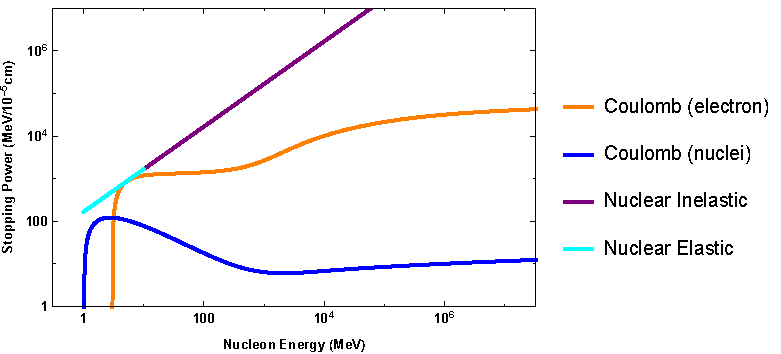
\includegraphics[scale=.60]{SPnucleon.pdf}
\caption{Nucleon energy loss in a WD with density $n_e = 10^{33} ~\text{cm}^{-3}$. The Coulomb stopping powers apply only to protons.}
\label{fig:SPnuc}
\end{figure}

\begin{figure}
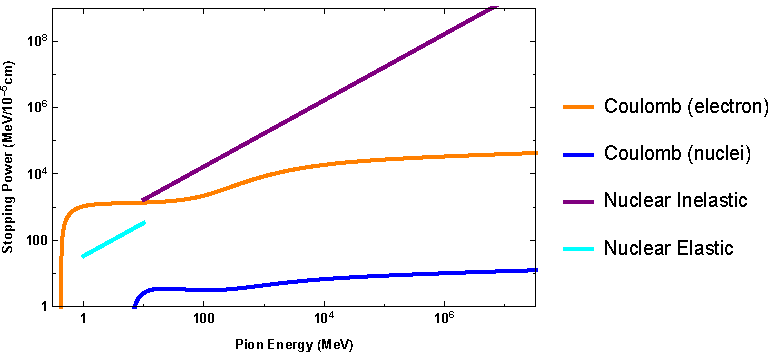
\includegraphics[scale=.60]{SPpion.pdf}
\caption{Pion energy loss in a WD with density $n_e = 10^{33} ~\text{cm}^{-3}$. The Coulomb stopping powers apply only to charged pion.}
\label{fig:SPpion}
\end{figure}

\subsection{Heating Properties: Electrons and Photons}
The stopping power of electrons and photons is highly sensitive to the density of the stellar medium.
This is evident in the fact that there is a critical density $n_e \sim 10^{32} ~\text{cm}^{-3}$ above which bremsstrahlung and pair production can essentially be ignored.
We begin by considering WD densities $n_e \lesssim 10^{32} ~\text{cm}^{-3}$.
The electron and photon energy loss functions for a density in this range are shown in Figures \ref{fig:SPelectron} and \ref{fig:SPphoton}.
In the case of both species, the dominant stopping mechanism at incident energies $\epsilon \sim 10^{3}-10^{5} ~\text{MeV}$ is due to electromagnetic radiative processes.
For an incident electron or photon of energy $\epsilon$, this will result in a cascade of secondary electrons and photons with typical shower length
\begin{equation}
X_\text{em} \sim \frac{2}{X_0} \l \l \frac{\epsilon}{E_\text{LPM}}\r^{1/2} - \l \frac{E_c}{E_\text{LPM}}\r^{1/2} \r,
\end{equation}
where $X_0$ is the radiation length and $E_\text{LPM}$ is the scale of LPM suppression, defined in Appendix \ref{sec:appendix}.
For an electromagnetic shower, $E_c \sim ~\text{TeV}$ is set by the energy at which Compton scattering dominates the stopping power.
At $\epsilon \sim 10^{5} ~\text{MeV}$, bremsstrahlung is suppressed by $\OO(\alpha)$ due to the LPM effect.

Therefore, at sufficiently high energies $\epsilon \gtrsim 10^5 ~\text{MeV}$ electrons and photons in the WD will lose energy primarily through nuclear interactions.
Effectively, electrons and photons at this energy behave like hadrons and will dump $\OO(1)$ of their initial energies into hadronic showers of length \eqref{eq:hadlength}.
However, the initial distance traversed to trigger a hadronic shower will vary between the two species.
For photons, this is roughly the photonuclear mean free path $l_\gamma$ while for electrons, the ``electronuclear radiation length" is found to be of order $\sim 10  ~l_\gamma/\alpha$.
Note that these initial length scales will dominate the overall size of $L_i$ as compared to the hadronic shower length.
In addition, $L_\text{electron}$ and $L_\text{photon}$ in this energy range also scale roughly linearly with WD density.
We now consider $n_e \gtrsim 10^{32} ~\text{cm}^{-3}$, for which radiative processes are negligible.
In this density regime, the stopping of electrons of incident energy $\epsilon \sim 1 - 10^4 ~\text{MeV}$ is primarily due to Coulomb collisions off degenerate electrons in the star.
At energies $\epsilon \gtrsim 10^4 ~\text{MeV}$, electronuclear and photonuclear processes become the dominant source of energy loss.

\subsection{Collective Heating by Many Particles}

\subsection{Summary of Standard Model Heating Channels}

To summarize, $L_i$ has been computed and plotted in Figure \ref{fig:cash} for the maximal WD density $n_e \sim 10^{33} ~\text{cm}^{-3}$ in the case of hadrons, electrons, and photons.
\textcolor{red}{caveat: we have not yet calculated the case of $\epsilon \lesssim 10^{5} ~\text{MeV}$ which proceeds through heating electrons.
This will result in a hot electron cloud after the shower distance $X_\text{em}$ that should ultimately thermalize ions.}

\begin{figure}
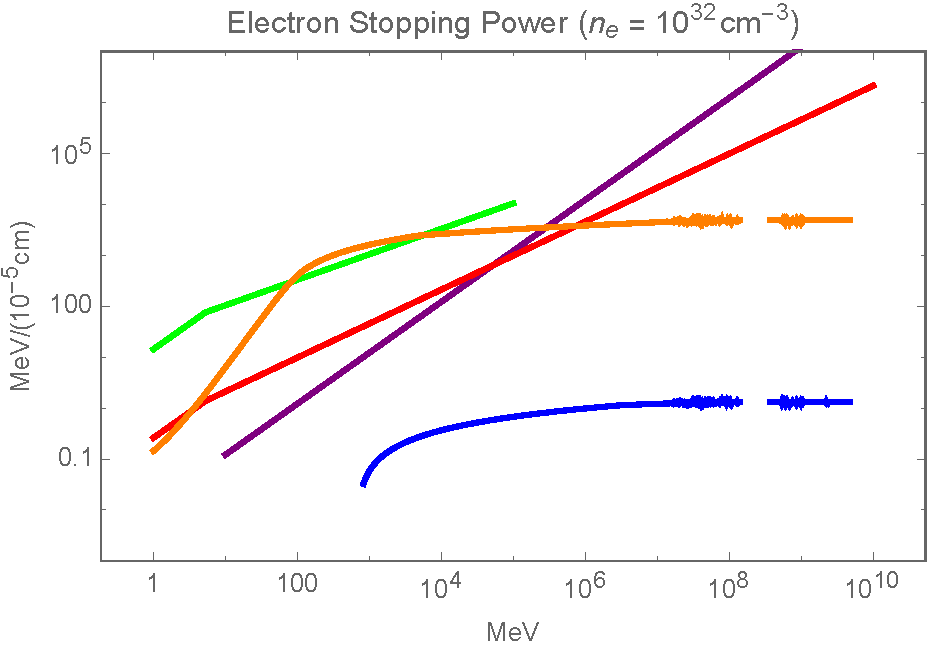
\includegraphics[scale=.60]{SPelectron.pdf}
\caption{Electron energy loss in a WD density $n_e = 10^{32} ~\text{cm}^{-3}$ For $n_e \gtrsim 10^{32} ~\text{cm}^{-3}$, bremsstrahlung and pair production contributions should be ignored}
\label{fig:SPelectron}
\end{figure}

\begin{figure}
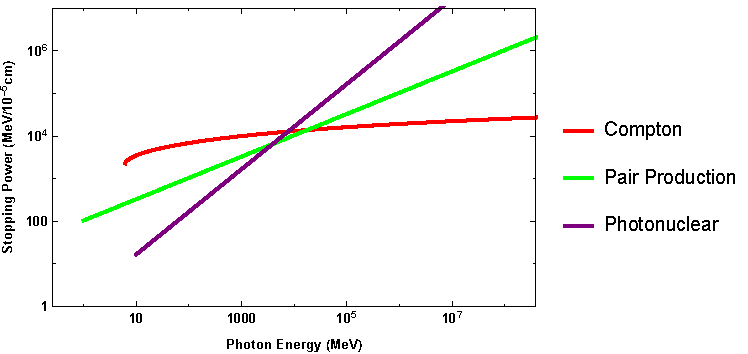
\includegraphics[scale=.60]{SPphoton.pdf}
\caption{Photon energy loss in a WD density $n_e = 10^{32} ~\text{cm}^{-3}$ For $n_e \gtrsim 10^{32} ~\text{cm}^{-3}$, bremsstrahlung and pair production contributions should be ignored}
\label{fig:SPphoton}
\end{figure}

\section{Dark Matter-Induced Ignition: Models and Conditions}
\label{sec:DMexplode}

In this section we discuss the DM-dependent aspects of heating WDs through SM secondaries produced from interactions as pictured in Figure \ref{fig:feynman}.
In particular, we parameterize the non-gravitational DM interactions that may give rise to WD heating in this fashion, discuss the typical spacial distributions of secondary particles that may be expected from such processes, and derive the conditions on the interaction parameters that determine if such encounters result in nuclear runaway.
Of course, these calculation in general require knowledge of model-dependent subtleties, particularly if the incoming DM particle is significantly effected by a collision with a carbon ion or if complex dark or SM states result from that interaction. 
In what follows, we specialize to three simple and illustrative types of DM-WD encounter that generically exist for ultra-heavy DM models: transits, collisions, and decays. 
The interactions giving rise to these encounters correspond to the diagrams shown in Figure \ref{fig:feynman}.


\subsection{DM-DM Collisions and DM Decays}
\label{sec:coldecay}
The collision of two DM states or the decay of a single DM within the WD is a generic interaction found in many models.
Note that these DM-DM collisions are not necessarily particle-antiparticle annihilations, but can be of a more general, complicated nature such as the collisions of heavy nuclei.
Since any such event will likely result in both SM and dark sector products, we parameterize the energy released into SM particles as a fraction $\eta$ of the DM mass.
Generically we might expect $\eta \ll 1$, although $\eta$ is at most unity for non-relativistic DM.
For simplicity, we restrict our attention to point-like events, where the SM products are produced near enough to the initial event site to give rise to a single temperature peak.
This excludes ``displaced vertex" events, whose explosion conditions would involve additional model-dependent parameters.
With this restriction, the explosion condition depends only on the total SM energy released and the heating length of the SM products $L_0$:
\begin{equation}
\label{eq:coldecay}
    m_\text{DM} \gtrsim \mathcal{E}_\text{boom} \cdot \frac{1}{\eta}
      \text{max}\left\{1, \frac{L_0}{\lambda_T}\right\}^3
\end{equation}
Considering the explosion threshold \eqref{eq:Eboom}, a DM-DM collision or DM decay requires masses larger than $\sim 10^{15} ~\GeV$ in order to release sufficient energy to trigger a SN.


\subsection{DM Transits}
\label{sec:transit}
For models with a DM-SM scattering interaction, there may be a continuous production of SM particles as the DM traverses a WD.
For simplicity, we consider the special case of a ``bullet-like" transit.
In such an encounter, DM penetrates the non-degenerate crust of a WD with negligible change in kinetic energy
\begin{align}
\label{eq:CrustCondition}
  \left( \frac{d E}{d x} \right)_\text{SP} \ll 
  \frac{m_\text{DM} v^2_\text{esc}}{R_\text{crust}},
\end{align}
where $R_\text{crust} \sim 50 ~\text{km}$ is the typical width of a WD crust, $v_\text{esc}$ is the the escape velocity of the WD, and $(dE/dx)_\text{SP}$ parametrizes the kinetic energy loss of the DM per distance travelled (i.e., the \emph{stopping power}).
Note that we have conservatively estimated the crust density to be roughly $\OO(1)$ of the interior density.
We define a transit event in terms of the WD crust since runaway fusion can only occur via heating of the degenerate stellar interior.
If condition \eqref{eq:CrustCondition} were not satisfied, then the kinematics of the DM transit would be highly dependent on details of the stopping power and must be calculated from a given model.
Instead, we avoid this complexity by imposing that the DM transits through a WD with approximately constant kinetic energy $\sim m_\text{DM} v^2_\text{esc}$.
Furthermore, since $R_\text{crust}$ will ultimately be larger than any of the heating lengths considered, we may also ignore energy loss within the WD interior.


The ability for a transit to ignite a star can be parameterized by a \emph{linear energy transfer} $(dE/dx)_\text{LET}$, which is the energy released into SM products per distance traveled.
Note that while the LET and stopping power are conceptually related quantities and may be equal in important special cases, they are generically different.
For a transit releasing high-energy particles with characteristic heating length $L_0$ per collision, the encounter can be broken up into a series of heating events of energy $\Ez = L_0 (d E/d x)_\text{LET}$.
If any individual deposition satisfies \eqref{eq:boom}, then runaway fusion obviously occurs.
If not, a SN may still be triggered due to the combined effect of many deposits.
In this scenario a large number of nearby temperature peaks will each diffuse outward, merging into a temperature profile that eventually satisfies \eqref{eq:boom}.
This is only relevant if $L_0 < \lambda_T$, in which case it is sensible to consider the combined deposit as a single heating event of length $\lambda_T$ and energy $\lambda_T (d E/d x)$.
However, such a coherent addition of individual energy deposits is only valid if the DM transit time is smaller than the relevant thermal evolution timescale.
The latter is dominated by the diffusion time $\tau_d$ across a distance $\lambda_T$ at temperature $T_f$.
Thus we require
\begin{align}
\tau_d \sim \frac{\lambda_T^2}{\alpha(T_f)} \gg \frac{\lambda_T}{v_\text{esc}},
\label{eq:SlowDiffusion}
\end{align}
where $\alpha(T_f)$ is the temperature-dependent diffusivity.
This condition is independent of DM model and has been checked to be satisfied for all WD densities.
Therefore, the explosion condition for transits satisfying \eqref{eq:CrustCondition} and \eqref{eq:SlowDiffusion} is given by
\begin{equation}
\label{eq:transitexplosion}
  \left( \frac{d E}{d x} \right)_\text{LET} \gtrsim n_\text{ion} T_f\, \text{max}\left\{\lambda_T, L_0 \right\}^2.
\end{equation}

\section{Constraints}
\label{sec:Constraints}

In this section we constrain generic ultra-heavy DM models that can interact with a WD to trigger runaway fusion.
Following the discussion of \cite{Graham:2015apa}, these constraints will come from (1)~the existence of heavy, long-lived white dwarfs and (2)~the measured type Ia SN rate.
In particular, both classes of observation will be affected if the DM of the universe were capable of igniting WDs via one the processes described in Section \ref{sec:DMexplode}.

The typical age of a WD is of order the age of the universe $\sim \text{Gyr}$.
RX~J0648.04418 is a nearby star and one of the heaviest known white dwarfs with a mass $\sim 1.25 ~M_{\odot}$.
From the WD mass-radius relation, we find the radius for such a star is $R_\text{WD} \approx 3000~\text{km}$ and the stellar escape velocity $v_\text{esc} \approx 4 \times 10^{-2}$.
Of course, this is not the only known heavy WD.
For instance, the Sloan Digital Sky Survey has found $\sim 20$ others \textcolor{blue}{get citation from SR}.
In fact, the NuStar collaboration has recently uncovered evidence for the likely existence of $\sim 1.25 ~M_{\odot}$ white dwarfs in the galactic center as well.
Such candidates are particularly suited for our constraints as the energy deposit needed to trigger supernova is a strong function of WD mass.

However, less dense white dwarfs are significantly more abundant in the galaxy.
Thus, even if a sufficiently massive DM is unable to trigger a violent heating event within the lifetime of a WD, it could still ignite enough lighter WDs to affect the measured SN rate of $\sim $ 0.3 per century.
The DM-induced SN rate is estimated using the expected number of white dwarfs per galaxy $\sim 10^{10}$ and their mass distribution \textcolor{blue}{get bib citations from SR}.
Simulations indicate that only WD masses heavier than $\sim 0.85 ~M_{\odot}$ will result in optically visible SN.
Therefore, most of the stars exploded in this manner will be in the mass range $\sim 0.85 - 1 ~M_{\odot}$, resulting in weaker SN than expected of typical Chandrasekhar WDs.

In summary, a bound on DM parameters can be placed if either a single explosive event occurs during the lifetime of an observed star such as RX~J0648.04418 or a possible heavy WD in the galactic center, or the SN rate due to such DM events throughout the galaxy exceeds the measured value.
The former condition can be viewed as a ``flux is too low" fundamental limit for the WD detector, while the latter can be viewed as a ``detection threshold" for signal over background.

\subsection{Collision and Decay Constraints}
\label{sec:CollisionConstraints}
The number of DM particles contained in a WD volume is approximately $\sim n_\text{DM} R_\text{WD}^3 (v_\text{esc}/v)$, taking into account the gravitationally enhanced DM number density within the star.
$v \sim 10^{-3}$ is simply the virial velocity of DM.
\textcolor{red}{of same order in galactic center?} Therefore, the expected DM-DM collision rate parameterized by cross section $\sigma_\text{DM-DM}$ is 
\begin{equation}
\Gamma_\text{collision} \sim \l \frac{\rho_{\text{DM}}}{m_\text{DM}} \r^2 \sigma_\text{DM-DM} \l \frac{v_\text{esc}}{v}\r^3 v R_\text{WD}^3,
\label{eq:collisiongamma}
\end{equation}
where $\rho_{\text{DM}}$ is the energy density of DM in the region of interest.
For a nearby star we take $\rho_\text{DM} \sim 0.4 ~\GeV/\text{cm}^3$, while for the white dwarfs observed in the galactic center we assume $\rho_\text{DM} \sim 10^3 ~\text{GeV}/\text{cm}^3$.
Likewise, the rate at which a single DM decay event occurs in the WD is
\begin{equation}
\Gamma_\text{decay} \sim  \frac{1}{\tau_\text{DM}} \frac{\rho_{\text{DM}}}{m_\text{DM}} \l \frac{v_\text{esc}}{v} \r R_\text{WD}^3,
\label{eq:taugamma}
\end{equation}
where $\tau_\text{DM}$ is the mean lifetime of DM.

In order for a collision or decay to trigger runaway fusion, it must release sufficient energy into SM particles.
Here we focus on a simple scenario wherein such a process releases a number of SM particles $N_i$ of single species $i$ and energy $\epsilon$ in a point-like event.
Each particle will deposit its energy and thermalize ions within a heating length $L_i (\epsilon)$, which was explicitly calculated in Section \ref{sec:SMHeating} for hadrons, electrons, and photons.
We are able to constrain DM interaction parameters when the collision or decay releases total energy greater than the threshold $\eqref{eq:coldecay}$.
If we assume a fractional parameter $\eta=1$, this corresponds to the entire mass of DM being converted into SM particles $i$, each with energy $m_\text{DM}/N_i$.
At sufficiently large $\epsilon \gtrsim \text{TeV}$, it has been shown that the heating lengths of individual SM particles only varies logarithmically in energy, independent of the species $i$.
Therefore, we treat $\epsilon$ as a free parameter whose precise value in the range $\epsilon \gtrsim \text{TeV}$ does not qualitatively modify the limits imposed.
In this case, $N_i$ and $\epsilon$ can both be fixed to the value at which $N_i \epsilon$ is of order $m_\text{DM}$ without affecting the nature of the constraints.
The only caveat in this scenario is that the value of $L_i (\epsilon)$ extrapolated to energies beyond $\sim 10^{17} ~\GeV$ must be done with caution.
As a result, for $m_\text{DM}$ greater than this scale, one can simply impose $\epsilon \lesssim 10^{17} ~\GeV$ with the number of released particles necessarily $N_i > 1$.

Of course, if the energy deposit required to trigger a supernova is greater than $\eqref{eq:coldecay}$ but still less than $\sim 10^{17} ~\GeV$, then it is possible that a single particle containing this energy is sufficient.
This is especially intriguing when we consider collisions or decays that release energy predominantly into neutrinos.
Neutrinos interact very weakly, although their nuclear cross section generically rises with energy.
A highly conservative estimate of this cross section in the energy regime of interest $\sigma_{\nu N} \sim 10^{-34} ~\text{cm}^2$ would indicate a mean free path of order $\sim \text{m}$.
Evidently, the neutrino heating length is too large to consider multiple neutrino emissions within a region of size $\lambda_T$.
However, a single neutrino can be thought of as a displaced vertex of size $\sim \text{m}$ which subsequently transfers its energy into high-energy hadrons or charged leptons.
Therefore, any DM model which admits a annihilation or decay into neutrinos of energy greater than $\sim 10^{15} ~\text{GeV}$ can be constrained just as we are able to do for more strongly interacting SM species.

In Figures \ref{fig:collisionclasses}, \ref{fig:collisioneta}, and \ref{fig:collisionspecies}, we show the constraints on cross section $\sigma_\text{DM-DM}$ as a function of $m_\text{DM}$ using the different classes of observation available and for representative choices of $\eta$ and SM species $i$ released.
Similarly, this is done for the lifetime $\tau_\text{DM}$ in Figures \ref{fig:decayclasses}, \ref{fig:decayepsilon}, and \ref{fig:decayspecies}.

\begin{figure}
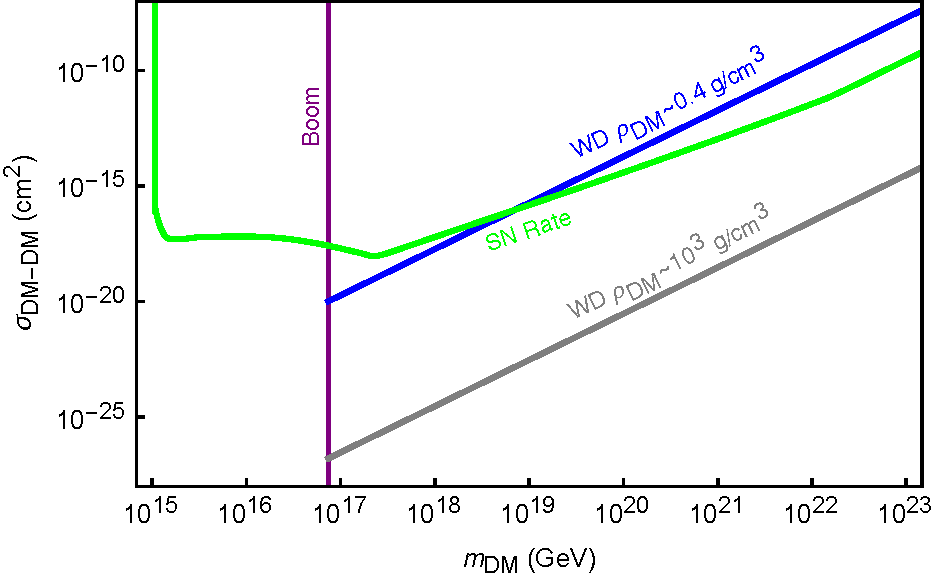
\includegraphics[scale=.45]{collisionobservation.pdf}
\caption{\textcolor{blue}{DM-DM collisions into photons with $\eta =1$, constrained using observations of a WD (local and galactic center) and measured SN rate}}
\label{fig:collisionclasses}
\end{figure}

\begin{figure}
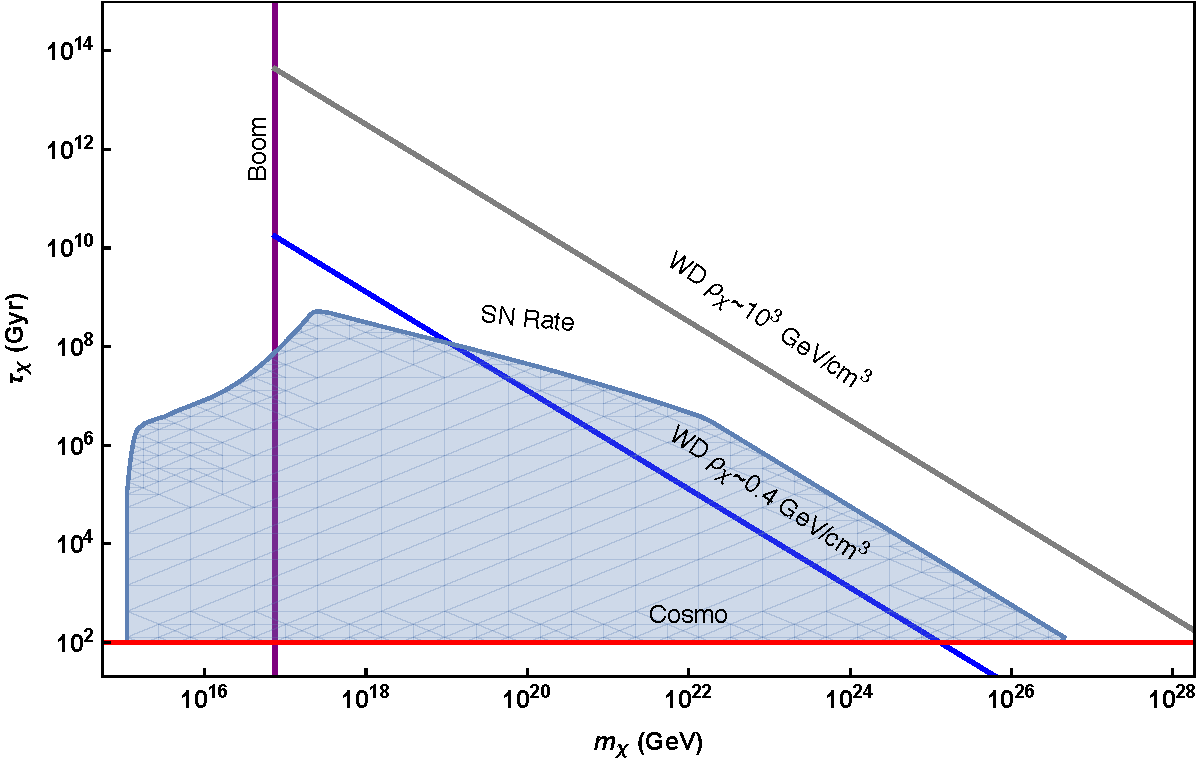
\includegraphics[scale=.45]{decayobservation.pdf}
\caption{\textcolor{blue}{DM decay into photons with $\eta =1$, constrained using observations of a WD (local and galactic center) and measured SN rate}}
\label{fig:decayclasses}
\end{figure}
 
\subsection{Transit Constraints}
\label{sec:TransitConstraints}

The DM transit rate through a WD (including a gravitational Sommerfeld enhancement) is given by
\begin{align}
\Gamma_\text{transit} \sim \frac{\rho_{\text{DM}}}{m_\text{DM}} R_\text{WD}^2 \l\frac{v_\text{esc}}{v}\r^2 v.
\label{eq:TransitFluxCondition}
\end{align}
Note that unlike \eqref{eq:collisiongamma} or \eqref{eq:taugamma}, the transit rate only depends on the DM mass.
We find that $m_\text{DM} \lesssim 10^{44} ~\GeV$ will transit a $1.25 ~M_{\odot}$ WD at least once in a Gyr.
This upper bound improves to $m_\text{DM} \lesssim 10^{44} ~\GeV$ in the case of a $1.25 ~M_{\odot}$ WD in the galactic center.

For a DM candidate to be constrained through its transit interaction with a WD, we demand that it penetrate the crust \eqref{eq:CrustCondition} and satisfy the explosive condition \eqref{eq:transitexplosion}.
As shown in Section \ref{sec:DMexplode}, a general DM transit is described by a stopping power and LET.
The former parameterizes the extent to which the DM slows down in the WD by losing kinetic energy, while the latter parameterizes the ability for the DM to dump sufficient energy to the star in the form of SM particles.
Let $\sigma_{i,\epsilon}$ denote the cross section for DM to scatter off a stellar constituent, producing $N_i$ SM particles of species $i$ and each with kinetic energy $\epsilon$.
If this were the only available channel for the DM to deposit energy, then the LET rate could be written as
\begin{align}
\label{eq:schematicLET}
  \left( \frac{d E}{d x} \right)_\text{LET} = n_\text{ion} \cdot N_i \sigma_{i,\epsilon} \epsilon,
\end{align}
where we have now restricted to the case of nuclear collisions.
Of course, the LET rate for any realistic DM model would necessarily involve a sum over stellar targets along with species $i$ that could be produced, as well as an integral over the produced particle spectrum.
For simplicity, we will assume a schematic picture in which \eqref{eq:schematicLET} adequately describes the DM transit through a WD.
The heating length of any such interaction is simply $L_i(\epsilon)$, computed in Section~\ref{sec:SMHeating} for electrons, photons, and hadrons.
In addition, we make a sensible assumption that the stopping power and LET are equal - that is, the DM loses kinetic energy at the same rate as energy is deposited to the WD.
While such a statement is certainly not true for all DM models (such as the Q-ball, which liberates binding energy rather than transferring kinetic energy), it provides a useful benchmark to express constraints.
With this simplification, it is also interesting to note that combining \eqref{eq:schematicLET} with the transit explosion condition \eqref{eq:transitexplosion} yields a lower bound on $m_{\text{DM}}$ such that the DM is able to both penetrate the crust \emph{and} trigger an explosion:
\begin{align}
\label{eq:transitmass}
m_{\text{DM}} \gtrsim  T_f ~\text{max}\{\lambda_T, L\}^2 \l \frac{n_{\text{ion}} R_{\text{crust}}}{v_{\text{esc}}^2} \r.
\end{align}
In other words, if \eqref{eq:transitmass} were violated then the DM interaction is either not strong enough to ignite the WD or it is so strong that it has no chance to penetrate the crust and transit the interior.
This translates to a condition that the DM mass must be greater than $\sim 10^{29} ~\GeV$ - the WD detector has an incredibly efficient shield.
However, it is important to note that this bound is only applicable when the energy input to the WD is chiefly coming from the DM kinetic energy, rather than binding energy or other sources.

Within this schematic for the DM transit, we constrain the parameter $\sigma_{i,\epsilon} \epsilon$ as a function of DM mass $m_\text{DM}$ (for simplicity, we set $N_i = 1$).
This is done in Figures \ref{fig:transitclasses}, \ref{fig:transitepsilon}, and \ref{fig:transitspecies} using the different classes of observation available and for representative choices of $\epsilon$ and SM species $i$ released.

\begin{figure}
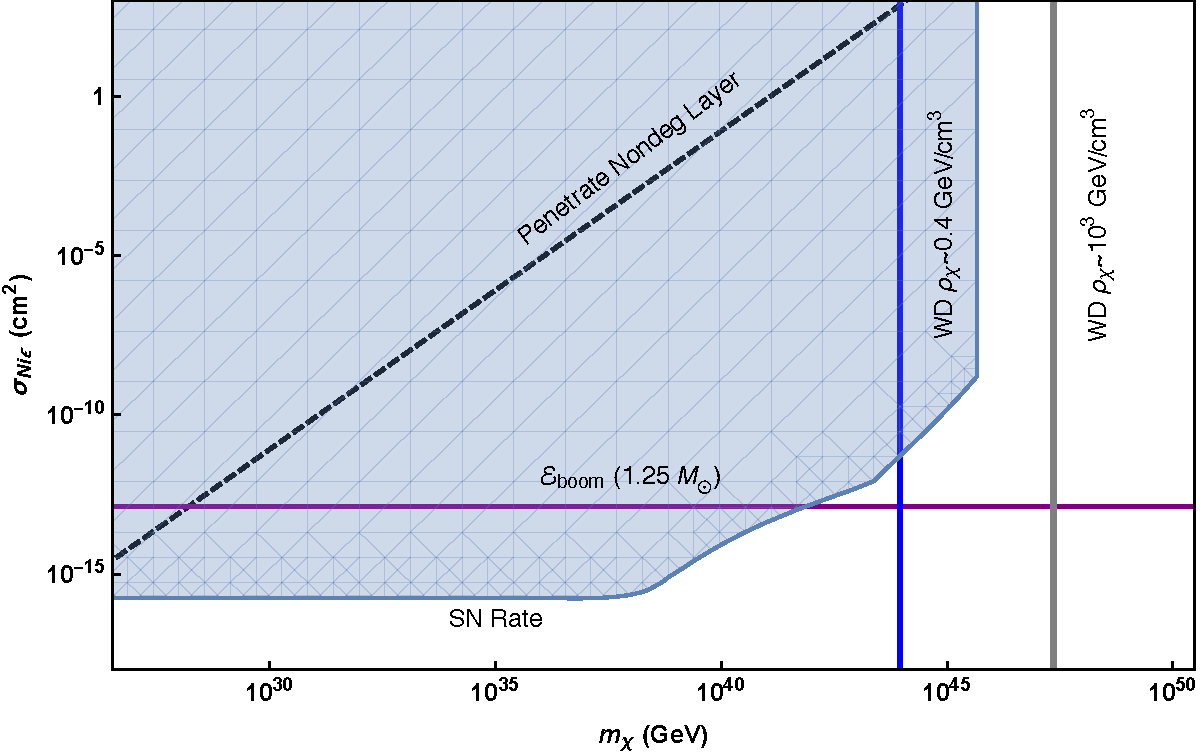
\includegraphics[scale=.45]{transitobservation.pdf}
\caption{\textcolor{blue}{Photons produced at $\epsilon = \text{TeV}$, constrained using observations of a WD (local and galactic center) and measured SN rate}}
\label{fig:transitclasses}
\end{figure}

\section{Q-balls}
\label{sec:QBalls}

We now implement the formalism for general constraints outlined in Section \ref{sec:Constraints} to place bounds on a specific model of DM: Q-balls.
In various supersymmetric extensions of the SM, non-topological solitons called Q-balls can be produced in the early universe \cite{Coleman:1985ki, Kusenko:1997si}.
If these Q-balls were stable, they would comprise a component of the DM today.

For gauge-mediated models with flat scalar potentials, the Q-ball mass and radius are given by
\begin{equation}
\label{eq:Qballprop}
M_Q \sim m_S Q^{3/4}, ~~~ R_Q \sim m_S^{-1} Q^{1/4},
\end{equation}
where $m_S$ is related to the scale of supersymmetry breaking.
The condition $M_Q/Q < m_p$ ensures that the Q-ball is stable against decay to nucleons \cite{Dine:2003ax}.
When an (electrically neutral) baryonic Q-ball interacts with a nucleon, it absorbs its baryonic charge as a minimum-energy configuration and induces the dissociation of the nucleon into free quarks.
During this process, $\sim \text{GeV}$ of energy is released through the emission of 2 - 3 pions \cite{Dine:2003ax}.
We assume that for each Q-ball collision, there is equal probability to produce $\pi^0$ and $\pi^\pm$ under the constraint of charge conservation.
The cross section for this interaction is approximately geometric:
\begin{align}
\sigma_Q \sim \pi R_Q^2.
\end{align}
Note that a sufficiently massive Q-ball will become a black hole if the Q-ball radius is less than the Schwarzschild radius $R_Q \lesssim G M_Q$.
In the model described above, this translates into a condition $(M_\text{pl}/m_S)^4 \lesssim Q$.
For Q-ball masses of this order, gravitational interactions become relevant.

We now summarize the explosiveness of a Q-ball transit.
According to the notation of Section \ref{sec:Constraints}, the Q-ball transit is described by an LET
\begin{align}
\left( \frac{d E}{d x} \right)^\text{Q-ball}_\text{LET} = N_\pi \cdot n_\text{ion} \sigma_Q \epsilon,
\end{align}
where the nuclear interaction results in $N_\pi \sim 30$ pions released, each with kinetic energy $\epsilon \sim 500 ~\text{MeV}$.
Numerous experiments have studied interactions of pions in this energy range incident upon complex nuclei targets such as carbon.
It is found that there is roughly equal cross section of order $\OO (100 ~\text{mb})$ for a (neutral or charged) pion to either elastically scatter or become absorbed in a nonelastic scatter with no final state pion \cite{Pionnuclear}.
As seen in Section \ref{sec:SMHeating}, nonelastic collisions are most relevant for energy loss and will induce a hadronic shower.
The corresponding heating length of the Q-ball interaction is computed in a straightforward manner
\begin{align}
L_0^\text{Q-ball} \sim \text{few} \times 10^{-7} ~\text{cm}
\end{align}
in WD density of $n_\text{ion} \sim 10^{32} ~\text{cm}^{-3}$.
If the Q-ball cross section is related to its mass and baryonic charge as in \eqref{eq:Qballprop}, we find that 
\begin{align}
Q \gtrsim 10^{38} \l\frac{m_S}{\text{TeV}}\r^4
\end{align}
is capable of triggering runaway fusion in a heavy $\sim 1.25 ~M_{\odot}$ WD.
Note that for such large values of $Q$ there is negligible stopping power for the Q-ball to slow down in a WD, and as such condition \eqref{eq:CrustCondition} will be trivially satisfied.

Currently, the strongest constraints on Q-balls come from large detectors, i.e. Super-Kamiokande as well as air fluorescence detectors of cosmic rays
However, the constraints possible with the WD detector are in a fundamentally inaccessible region of parameter space for these terrestrial-based experiments due to the extremely low flux, and thus our new constraints are wholly complementary.
The strongest proposed limits due to the existence of a heavy WD in the galactic center are plotted in Figure~\ref{fig:Qballconstraint}. As a comparison, the combined limits from Super-K and the OA,TA cosmic ray detectors are shown in red. 

\begin{figure}
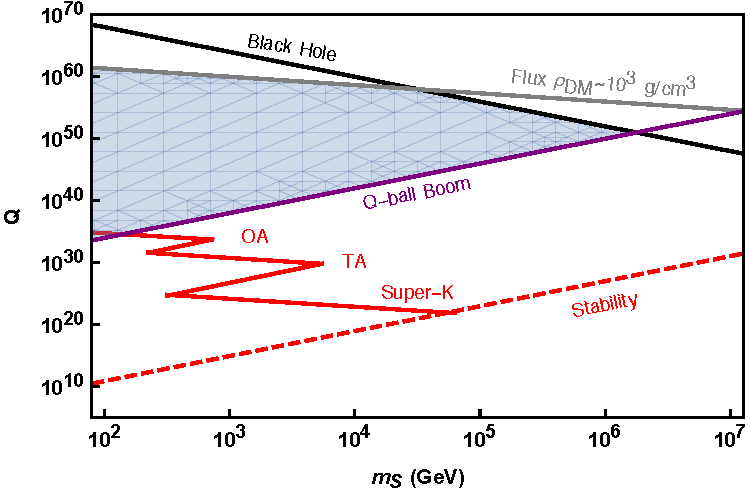
\includegraphics[scale=.45]{Qballconstraint.pdf}
\caption{Constraints on baryonic Q-balls from transits of a $\sim 1.25 ~M_{\odot}$ WD in the galactic center. Also shown are the limits from Super-K and the OA, TA cosmic ray detectors (red), and the lower bound on $Q$ for which the Q-ball is stable against decay to nucleons (black).}
\label{fig:Qballconstraint}
\end{figure}

\section{Discussion}
\label{sec:discussion}

\begin{appendices}

\section{Particle Interactions in a White Dwarf}
\label{sec:appendix}
In this appendix we provide a detailed analysis of the possible electromagnetic and strong interactions in a WD.
This is primarily aimed towards calculating the stopping of high-energy electrons, photons, and light hadrons (protons, neutrons, pions) within the stellar medium.
The interior of a WD is a complex environment (unless otherwise noted, we will assume a carbon-oxygen WD).
Famously, the star is supported against collapse by electron degeneracy pressure with a characteristic Fermi energy
\begin{equation}
E_F = (3 \pi^2 n_e)^{1/3} \sim 0.1 - 1 ~\text{MeV}
\end{equation}
where $n_e$ is the number density of electrons.
The nuclei are at an ambient temperature $T \sim \text{keV}$ and form a strongly-coupled plasma with lattice energy
\begin{equation}
\label{eq:lattice}
\omega \sim \frac{Z^2 \alpha}{n_\text{ion}^{-1/3}} \sim 10^{-2} - 10^{-1} ~\text{MeV}
\end{equation}
where $n_\text{ion}$ is the number density of nuclei \cite{Teukolsky}.

\subsection*{Coulomb Collisions}

An incident particle of mass $m$, charge $e$, and velocity $\beta$ scattering off a stationary target of mass $M$, charge $Ze$ at impact parameter $b$ will transfer energy
\begin{equation}
\label{eq:impact}
E' = \frac{2 Z^2 \alpha^2}{b^2 \beta ^2 M},
\end{equation}
valid for energy transfers less than the mass of the target. 
The differential cross section for the interaction is given by the Rutherford cross section
\begin{equation}
\label{eq:rutherford}
\frac{d \sigma}{dE'} = \frac{2 \pi  \alpha^2 Z^2}{M \beta^2} \frac{1}{E'^2},
\end{equation}
where we have assumed a sufficiently fast incident particle so that interactions are governed by single collisions with energy transfer $E'$ \cite{Agashe:2014kda}.
In the case of a target electron, the full QED calculation yields a cross section of the same form
\begin{equation}
\frac{d \sigma}{dE'} = \frac{2 \pi  \alpha^2 Z^2}{m_e \beta^2} \frac{1}{E'^2} \l1-\beta^2 \frac{E^\prime}{E_\text{kin}} \r,
\end{equation}
where $E_\text{kin}$ is the maximum possible energy transfer satisfying kinematic constraints in a backward scatter:
\begin{equation}
\label{eq:Ekin}
E_{\text{kin}} = \frac{2 m_e \beta^2 \gamma^2}{1+ 2\gamma m_e/m +(m_e/m)^2}
\end{equation}

It is straightforward to understand the parametric dependences of \eqref{eq:rutherford}: there is increased likelihood to scatter for slowly moving incident particles undergoing soft-scatters against lighter targets.
Therefore, one would expect that soft-scattering dominates the energy loss, and that collisions with nuclei of mass $M$ are suppressed by a factor $\OO\l\frac{Z m_e}{M}\r$ as compared to collisions with electrons.
This is certainly true for incident charged particles in non-degenerate matter.
However, both of these naive expectations turn out to be false when considering scattering off a degenerate species.

We first consider the energy loss of high-energy charged particles colliding with non-degenerate nuclear targets. 
In this case, the stopping power is given by:
\begin{align}
\label{eq:SP}
-  \frac{dE}{dx} \sim \frac{n_\text{ion} Z^2 \alpha^2}{M \beta^2} \log {\l\frac{E_{\text{max}}}{E_{\text{min}}}\r}.
\end{align}
We take the upper limit on energy transfer to be the kinematic bound \eqref{eq:Ekin}, while the the maximum impact parameter is set by Thomas-Fermi screening due to the degenerate electron gas:
\begin{equation}
\label{eq:TF}
\lambda_{\text{TF}} = \l \frac{6 \pi Z \alpha n_e}{E_F}\r^{-1/2}.
\end{equation}

However, for energy transfers greater than $\omega$, the lattice structure of ions in the WD introduces further complications.
Namely, momentum transfers from collisions below this threshold will lead to suppressed energy loss due to collective effects.
We set the lower bound on Coulomb scattering off nuclear targets (not applicable for electron targets) to be $\sim \omega$ so that we only account for energy transfers greater than the ion lattice binding energy.
At lower energies, we estimate the stopping power into phonon excitations as follows: \textcolor{blue}{paragraph on phonons?}

Now consider collisions with degenerate electrons.
While a proper treatment would also take into account the relativistic motion of the degenerate electron gas, such a calculation would only modify these results by $\OO(1)$ factors. 
An incident particle transferring energy $E'$ can only scatter those electrons within $E'$ of the Fermi surface.
We define a modified density of electrons $n_e(E')$ as:
\begin{equation}
\label{eq:pauliblocking}
n_e(E') = \left\{
        \begin{array}{ll}
            \displaystyle \int \limits_{E_F -E'}^{E_F}dE ~g(E) & \quad E_F \geq E' \\
            n_e & \quad E_F \leq E'
        \end{array}
    \right.,
\end{equation}
where $g(E)$ is the density of states per unit volume for a three-dimensional free electron gas.
The effect of degeneracy can also be cast as a suppression of the differential cross section of order $\mathcal{O}(E'/E_F)$ whenever energy less than the Fermi energy is transferred.
Therefore, unlike in the non-degenerate case, the energy loss due to soft-scatters are in fact subdominant to the contributions from rare hard-scatters.
The stopping power is also sensitive to the integration bounds $E_{\text{max}}$ and $E_{\text{min}}$ as a power-law dependence unlike the logarithmic sensitivity \eqref{eq:SP} in the case of a non-degenerate target.

\subsection*{Compton and Inverse Compton Scattering}
Photons and charged particles can elastically exchange energy via Compton scatters.
We focus first on an incident photon losing energy to the WD medium.
Since the cross section for this process scales inversely with the target mass, the stopping due to photon-ion collisions will be subdominant to photon-electron collisions and we ignore the former. 
Consider an incident photon of energy $k$ scattering off an electron of energy $E \sim E_F$.
In the rest frame of the electron, this cross section is given by the Klein-Nishina formula
\begin{equation}
\label{KN}
  \frac{d\sigma_\text{KN}}{d (\cos \theta)} = \frac{\pi \alpha^2}{m_e^2} 
  \l \frac{k^\prime}{k} \r^2 
  \l \frac{k^\prime}{k} + \frac{k}{k^\prime} -\sin^2 \theta \r
\end{equation}
where $k^\prime$ is the outgoing photon energy, related to the scattering angle $\theta$ by Compton's formula
\begin{equation}
{k^{\prime }={\frac {k}{1+{\frac {k}{m_e}}(1-\cos \theta )}}}.
\end{equation}
In the limit $k > m_e$, the cross section is suppressed by the incoming energy $\sigma \sim \frac{\alpha^2}{m_e k}$. 
The outgoing photons will scatter predominately in a near-forward direction, $\cos \theta \approx m_e/k$, with an energy loss $k^\prime \sim m_e$.
Thus the typical photon energy loss is large, $\Delta k \sim m_e - k$, and cooling proceeds via a small number of hard scatters.
The stopping power is roughly:
\begin{equation}
\label{eq:approx-comptonSP}
  -\frac{dk}{dx} \sim n_e \sigma \Delta{k} 
  \sim-n_e \frac{\alpha^2}{m_e} \l 1 - \frac{m_e}{k} \r
\end{equation}
which for $k \gg \MeV$ rapidly plateaus to
\begin{equation}
\label{eq:plateau-comptonSP}
  -\frac{dk}{dx} \sim n_e \frac{\alpha^2}{m_e} 
   \sim 100 \frac{\MeV}{10^{-5} \cm}.
\end{equation}
A more careful analysis computes the stopping power as 
\begin{equation}
\label{eq:comptonSP}
  \frac{dk}{dx} =  \int d (\cos \theta) n_e \frac{d\sigma_\text{KN}}{d (\cos \theta)} \l k - k^\prime \r, 
\end{equation}
taking into account the Lorentz boost to the electron's rest frame.
This does not alter the result beyond $\OO(1)$ factors, since the target electrons are only slightly relativistic.
Further, Pauli-blocking of the target electrons should be taken into account via \eqref{eq:pauliblocking}, although we find that degeneracy only introduces a significant suppression when $k \lesssim 10 ~\text{MeV}$.
This is also expected, as the interaction is dominated by hard, near-forward scatters.

We now briefly consider incident electrons which may cool by (inverse) Compton scatters with the thermal bath of photons in the WD.  
The number density of these photons is set by the thermal temperature of the star, $n_\gamma \sim T^3$, which for $T \sim \text{keV}$ gives $n_\gamma \sim 10^{23} \cm^{-3}$.
This is roughly ten orders of magnitude less dense than the ions and electrons in the medium, so this interaction is expected to always be negligible compared to electron-ion or even electron-electron scattering.
An estimate in the manner of the above calculation (including the now-significant boost factors) gives the inverse Compton stopping power in terms of the photon temperature $T$ and incident electron energy $E$:  
\begin{equation}
\label{eq:invcomptonSP}
  -\frac{dE}{dx} \sim 
  \begin{cases}
    \alpha^2 \frac{T^4}{m_e^4} E^2 & E < \frac{m_e^2}{T} \\
    \alpha^2 T^2 & E > \frac{m_e^2}{T} \\
  \end{cases},
\end{equation}
where the change in scaling with $E$ marks a transition from Thompson-like scattering in the electron rest frame to suppressed high-energy scattering.
This stopping power plateaus at roughly $5\cdot10^{-3}\,\MeV/(10^{-5} \cm)$, which is indeed negligible. 

\subsection*{Bremsstrahlung and Pair Production with LPM Suppression}
Bremsstrahlung and pair production can be significant sources of energy loss for high-energy electrons and photons. We restrict our attention to radiative processes off target nuclei rather than target electrons as the latter are additionally suppressed by degeneracy, kinematic recoil, and charge factors. 
The cross section for an electron of energy $E$ to radiate a photon of energy $k$ is given by the Bethe-Heitler formula
\begin{equation}
\label{eq:BH}
\frac{d \sigma_\text{BH}}{dk} = \frac{1}{3 k n_\text{ion} X_0} (y^2+2 [1+ (1-y)^2]), ~~~ y = k/E.
\end{equation}
$X_0$ is the radiation length, and is generally of the form
\begin{equation}
\label{eq:radiationlength}
X_0^{-1} = 4 n_\text{ion} Z^2 \frac{\alpha^3}{m_e^2} \log{\Lambda}, ~~~ \log{\Lambda} \sim \int \limits_{b_\text{min}}^{b_\text{max}} \frac{1}{b}.
\end{equation}
where $\log{\Lambda}$ is a logarithmic form factor containing the maximum and minimum effective impact parameters allowed in the scatter.
Integrating \eqref{eq:BH}, we find the energy loss due to bremsstrahlung is simply 
\begin{equation}
-\frac{dE}{dx} \sim \frac{E}{X_0}.
\end{equation}

$b_\text{min}$ in \eqref{eq:radiationlength} is set by a quantum-mechanical bound such that the radiated photon frequency is not larger than the initial electron energy. 
For a bare nucleus, this distance is the electron Compton wavelength $b_\text{min} = \lambda_e = \frac{1}{m_e}$. \textcolor{blue}{another sentence to clarify}
It is important to note that collisions at impact parameters \emph{less} than $b_\text{min}$ will still radiate, but with exponentially suppressed intensity.
Classically, this is manifested by the decoherence of radiation at large scattering angles.
$b_\text{max}$ is set by the distance at which the nuclear target is screened.
For an atomic target this is of order the Bohr radius, and in the WD this is the Thomas-Fermi length \eqref{eq:TF}.
Evidently, there exists a critical electron number density $n_e \sim 10^{32} ~\text{cm}^{-3}$ at which the logarithmic form factor vanishes.
For our purposes, we simply take $\log{\Lambda} \sim \OO(1)$ whenever $b_\text{min} \lesssim b_\text{max}$ while effectively ignoring the energy loss due to bremsstrahlung in a sufficiently dense WD.

However, bremsstrahlung will be suppressed by the ``Landau-Pomeranchuk-Migdal" (LPM) effect - see \cite{Klein:1998du} for an extensive review.
High-energy radiative processes involve very small longitudinal momentum transfers to nuclear targets ($\propto k/E^2$ in the case of bremsstrahlung).
Quantum mechanically, this interaction is delocalized across a formation length over which amplitudes from different scattering centers will interfere.
This interference turns out to be destructive and must be taken into account in the case of high energies or high-density mediums.
Calculations of the LPM effect can be done semi-classically based on average multiple scattering.
It is found that bremsstrahlung is suppressed for $k < E(E-k)/E_\text{LPM}$, where
\begin{equation}
\label{eq:LPM}
E_\text{LPM} = \frac{m_e^2 X_0 \alpha}{4 \pi}.
\end{equation}
For the WD densities in which radiative energy loss is considered, $E_\text{LPM} \sim 10-10^{3} ~\text{MeV}$.
The degree of suppression is found to be
\begin{equation}
\frac{d\sigma_\text{LPM}/dk}{d\sigma_\text{BH}/dk} = \sqrt{\frac{k E_\text{LPM}}{E (E-k)}},
\end{equation}
so that the bremsstrahlung stopping power in the regime of high-suppression is modified
\begin{equation}
\label{eq:bremloss}
-\l\frac{dE}{dx}\r_\text{LPM} \sim \l\frac{E_\text{LPM}}{E} \r^{1/2} \frac{E}{X_0}, ~~~ E>E_\text{LPM}.
\end{equation}
We find that the LPM effect diminishes energy loss due to soft radiation so that the radiative stopping power is dominated by single, hard bremsstrahlung.

In addition to the LPM effect, other forms of interaction within a formation length will suppress bremsstrahlung when $k \ll E$.
The emitted photon can coherently scatter off electrons and ions in the media, acquiring an effective mass of order the plasma frequency $\omega_p$.
Semi-classically, this results in a suppression of order $(k/\gamma \omega_p)^2$ when the radiated photon energy $k < \gamma \omega_p$.
This is known as the ``dielectric effect".
For high-energy electrons, this dielectric suppression only introduces a minor correction to \eqref{eq:bremloss}, in which soft radiation is already suppressed by the LPM effect \cite{Klein:1998du}.

We now briefly summarize the stopping of photons via pair production. Similar to \eqref{eq:BH}, the cross section for a photon of energy $k$ to produce an electron-positron pair with energies $E$ and $k-E$ is
\begin{equation}
\label{eq:PP}
\frac{d \sigma_\text{BH}}{dE} = \frac{1}{3 k n_\text{ion} X_0} (1+ 2[x^2+ (1-x)^2]) ~~~ x = E/k,
\end{equation}
valid beyond the threshold energy $k \gtrsim m_e$. 
As a result, the pair production cross section $\sim 1/(n_\text{ion} X_0)$.
However, the LPM effect suppresses pair production at energies $E(k-E) > k E_\text{LPM}$ so that the cross section reduces to
\begin{equation}
\sigma_{pp} \sim \l\frac{E_\text{LPM}}{k} \r^{1/2} \frac{1}{n_\text{ion} X_0}, ~~~ E>E_\text{LPM}.
\end{equation}

Note that the LPM effect is less significant for higher-order electromagnetic processes since these generally involve larger momentum transfers for the same final-state kinematics.
Thus, when the suppression factor exceeds $\OO(\alpha)$, these interactions should also be considered.
For instance, the energy loss due to electron direct pair production $e^-N \to e^+ e^- e^- N$ has been calculated in \cite{Gerhardt:2010bj} and is found to exceed that of bremsstrahlung at an energy $\sim 10^{8} ~\GeV$. 
A similar crossover is to be expected for other higher-order diagrams as well, although such a calculation is beyond the scope of this work. 
Rather, it is expected that at such high energies the stopping power is dominated by photonuclear and electronuclear interactions anyway, and we may simply ignore the contributions from other radiative processes. 

\subsection*{Nuclear Interactions}
Nuclear interactions can be either elastic or nonelastic - the nature of the interaction is largely determined by the incident particle energy.
Elastic collisions are most relevant at scales less than the nuclear binding energy, $E_\text{nuc} \sim 10 ~\text{MeV}$.
A single, backward elastic scatter could result in an incident particle losing virtually all of its energy if the incident and target masses are the same.
However, we will be primarily concerned with light hadrons incident on relatively heavy nuclei, i.e.
ping-pong balls bouncing around a sea of bowling balls.

An elastic collision between an incident (non-relativistic) mass $m$ and a heavy, stationary target mass $M$ results in a final energy
\begin{equation}
\label{eq:elasticratio}
\zeta \equiv \frac{\epsilon'}{\epsilon} \approx \l \frac{M}{M+m} \r^2, ~~~~ m < M.
\end{equation}
$\epsilon$ and $\epsilon'$ denote the initial and final energy of the incident particle, and we assume an isotropic distribution in the center-of-mass scattering angle.
Thus, a nucleon interacting with carbon nuclei transfers roughly 15\% of its incident energy after each elastic collision.
However, since the ions in a WD form a Coulomb lattice, elastic collisions cannot transfer energy less than \eqref{eq:lattice} without exciting phonon modes.
In the case of a nucleon, this limits the applicability of \eqref{eq:elasticratio} to energies $\epsilon \gtrsim \text{MeV}$.

The cross section for elastic scatters $\sigma_\text{el}$ has considerable dependence on the incident particle species and energy.
At energies below $\sim \text{MeV}$, $\sigma_\text{el}$ effectively vanishes for protons.
In the case of neutrons, $\sigma_\text{el}$ is roughly constant below $\sim \text{MeV}$ but is of a complicated form in the intermediate regime $1 - 10 ~\text{MeV}$ due to various nuclear resonances \textcolor{blue}{cite ENDF}.
For our purposes, we assume the elastic cross section for any hadron to be constant $\sigma_\text{el} \sim 1 ~\text{b}$ when $\epsilon \gtrsim \text{MeV}$.

Next we consider nonelastic collisions at incident energies $\epsilon \gtrsim E_\text{nuc}$.
In this regime, a nuclear collision generally results in an $\OO(1)$ number of energetic secondary hadrons (i.e.
protons, neutrons, pions, etc.) emitted roughly in the direction of the primary particle.
These secondary particles approximately split the initial total energy of the absorbed primary particle and can collide with other nuclei in the WD.
The remnant nucleus will generally be left in an excited state and relax through the emission of $\OO(10 ~\text{MeV})$ hadrons (``nuclear evaporation") and photons \cite{Rossi}.
A hadronic shower is the result of all such reactions caused by primary and secondary particles.

For simplicity, we take the nuclear mean free path for a light hadron (proton, neutron, pion) to be constant in energy with characteristic cross section
\begin{equation}
l_\text{h,inel} \sim  \frac{1}{n_\text{ion} \sigma_\text{non}}, ~~~~ \sigma_\text{non} \sim 100 ~\text{mb}.
\end{equation}
Note that the shower length is only logarithmically sensitive to the initial energy or number of secondaries, and is thus primarily set by the nuclear mean free path.
In this case, the cascade induced by a high-energy initial hadron is adequately described by a stopping power
\begin{equation}
\label{eq:nucshower}
-\l \frac{dE}{dx}\r_\text{had} \sim \frac{E}{l_\text{h,inel}},
\end{equation}
neglecting logarithmic factors of $\OO(1)$.
The shower will end once final-state hadrons reach a critical energy $E_c$ - this is either the scale at which an additional mechanism dominates the stopping power or the minimum energy required to induce further showers $E_\text{nuc}$.
Note that while neutrons and $\pi^\pm$ have characteristically long lifetimes, the mean distance traversed by a neutral pion before decaying to photons $d_{\pi^0} = \gamma v \tau \approx 10^{-7} - 10^{-6} ~\text{cm}$ for $\epsilon \sim 1 - 10 ~\text{MeV}$.
For the most dense WD under consideration, the nuclear mean free path for a nonelastic collision is roughly $l_\text{h,inel} \approx 10^{-7} \text{cm}$.
Hence, there are minimal electromagnetic contributions from $\pi^0$ decays during the progression of a hadronic cascade.

Energetic $k \gtrsim 10 ~\text{MeV}$ photons can also interact with nuclei and induce a hadronic shower.
There is considerable uncertainty in the evaluation of high-energy photonuclear cross sections, and a detailed model is beyond the scope of this work.
In fact at sufficiently high energies, photonuclear interactions can become coherent with the photon interaction spread over multiple nuclei \cite{Gerhardt:2010bj}.
This coherence will further reduce the photonuclear mean free path.
As a conservative estimate, \textcolor{blue}{neglecting the $k^{0.08}$ dependence at high energies} we assume a constant photonuclear cross section in the relevant energy regime
\begin{equation}
l_\gamma \sim \frac{1}{n_\text{ion} \sigma_{\gamma A}}, ~~~~ \sigma_{\gamma A} \sim 1 ~\text{mb}.
\end{equation}

Similarly, charged leptons will lose energy via electronuclear interactions in which the incident particle radiates a virtual photon that then interacts hadronically with a nearby nucleus.
Note that a hadronic shower induced by electronuclear interactions are not affected by the LPM suppression \eqref{eq:LPM}.
Naively we expect the stopping power to be of order $\sim E \alpha/l_\gamma$.
A more detailed calculation \cite{Gerhardt:2010bj} differs from our naive estimate an $\OO(10)$ factor.
The largest uncertainty in calculating electronuclear stopping power at high energies is in evaluating hadronic cross sections, which require significant extrapolation from existing data and for which different models yield different results.

\end{appendices}

\section*{Acknowledgements}
We would like to thank D.Grabowska, K.Harigaya, S.R.Klein, R.McGehee, and J.Wurtele for stimulating discussions.
\textcolor{blue}{Grant acknowledgements}

\bibliography{Qballs}

\end{document}
